\documentclass[border=10pt]{standalone}
\usepackage{tikz}
\usetikzlibrary{arrows.meta}

\begin{document}
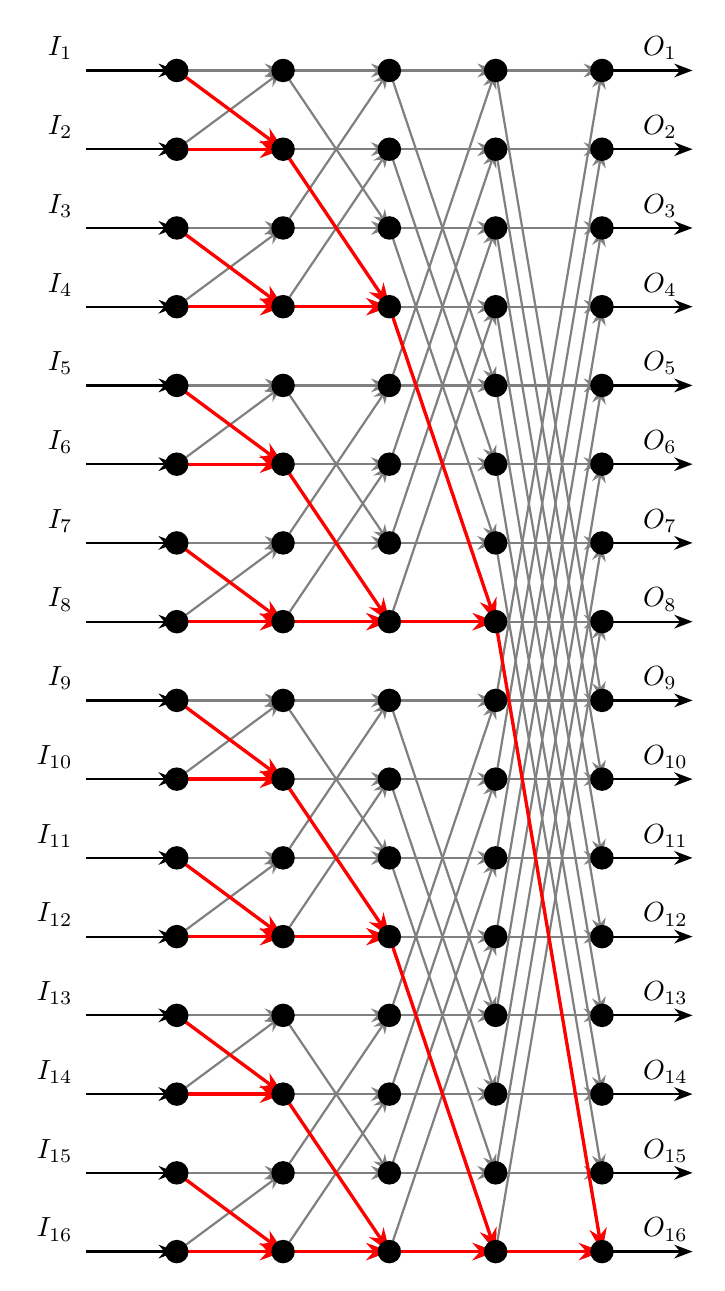
\begin{tikzpicture}[>=Stealth]

% Define styles
\tikzset{
    node/.style={circle, fill=black, inner sep=3pt},
    redarrow/.style={->, red, line width=1.2pt},
    grayarrow/.style={->, gray, line width=0.8pt},
    blackarrow/.style={->, black, thick}
}

% Column coordinates: input, three internal columns, output
\foreach \r in {1,...,16} {
    \coordinate (P0-\r) at (0,-\r);
    \coordinate (P1-\r) at (1.35,-\r);
    \coordinate (P2-\r) at (2.70,-\r);
    \coordinate (P3-\r) at (4.05,-\r);
    \coordinate (P4-\r) at (5.40,-\r);
}

% External input and output arrows with labels
\foreach \i in {1,...,16} {
    \draw[blackarrow] (-1.15,-\i) -- (P0-\i);
    \node[left=0.25cm] at (-0.95,-\i+0.28) {$I_{\i}$};
}
\foreach \o in {1,...,16} {
    \draw[blackarrow] (P4-\o) -- (6.55,-\o);
    \node[right=0.25cm] at (5.55,-\o+0.28) {$O_{\o}$};
}

% Gray butterfly-style connections between every adjacent column
\foreach \c/\off in {0/1,1/2,2/4,3/8} {
    \pgfmathtruncatemacro{\nextc}{\c+1}
    \pgfmathtruncatemacro{\block}{2*\off}
    \foreach \r in {1,...,16} {
        \pgfmathtruncatemacro{\m}{mod(\r-1,\block)}
        \ifnum\m<\off
            \pgfmathtruncatemacro{\p}{\r+\off}
        \else
            \pgfmathtruncatemacro{\p}{\r-\off}
        \fi
        \draw[grayarrow] (P\c-\r) -- (P\nextc-\r);
        \draw[grayarrow] (P\c-\r) -- (P\nextc-\p);
    }
}

% Red highlighted converging butterfly paths ending at O16
\foreach \e in {2,4,...,16} {
    \pgfmathtruncatemacro{\a}{\e-1}
    \draw[redarrow] (P0-\a) -- (P1-\e);
    \draw[redarrow] (P0-\e) -- (P1-\e);
}
\foreach \e in {4,8,12,16} {
    \pgfmathtruncatemacro{\a}{\e-2}
    \draw[redarrow] (P1-\a) -- (P2-\e);
    \draw[redarrow] (P1-\e) -- (P2-\e);
}
\foreach \e in {8,16} {
    \pgfmathtruncatemacro{\a}{\e-4}
    \draw[redarrow] (P2-\a) -- (P3-\e);
    \draw[redarrow] (P2-\e) -- (P3-\e);
}
\draw[redarrow] (P3-8) -- (P4-16);
\draw[redarrow] (P3-16) -- (P4-16);

% Draw black nodes on top of the arrows
\foreach \i in {1,...,16} {
    \node[node] (I\i) at (P0-\i) {};
    \node[node] (N1-\i) at (P1-\i) {};
    \node[node] (N2-\i) at (P2-\i) {};
    \node[node] (N3-\i) at (P3-\i) {};
    \node[node] (O\i) at (P4-\i) {};
}

\end{tikzpicture}
\end{document}
